\documentclass[a4paper, 11pt]{article}
\usepackage[margin=1in]{geometry}
\usepackage{amsmath}
\usepackage{graphicx}
\usepackage{tikz}
\usepackage[hidelinks]{hyperref}
\usepackage{color}
\usepackage{xcolor}
\usepackage{listings}
\usepackage{float}
\usepackage{setspace}

%\renewcommand{\baselinestretch}{1.5}

\lstset{basicstyle=\small}

\usepackage{caption}
\DeclareCaptionFont{white}{\color{white}}
\DeclareCaptionFormat{listing}{\colorbox{gray}{\parbox{\textwidth}{#1#2#3}}}
\captionsetup[lstlisting]{format=listing,labelfont=white,textfont=white}

\begin{document}
%Header-Make sure you update this information!!!!
\noindent
\large\textbf{Obligatory Assignment 2 Report} \hfill \textbf{Tomasz Gliniecki} \\


\section*{Problem 1}
System works if at least 11 components work.

\emph{Simulation}:
\\

\centerline{$ \sum_{i=1}^{15} I (U_i \leq p_i) \geq 11 $}

\subsection*{a)}
analytical\\
\centerline{$1+\sum_{i=0}^{10} - \binom{15}{i} 0.1^{15-i} 0.9^i = 0.987 $}
simulation results:\\
\centerline{P(System works) = $ 0.987 $}

\subsection*{b)}

\centerline{with probabilities: $.9, .9, .7, .8, .8, .7, .9, .7, .7, .8, .8, .7, .9, .8, .9, .8$}

\begin{lstlisting}
p <- c( .9, .9, .7, .8, .7, .9, .7, .7, .8, .8, .7, .9, .8, .9, .8 )
n <- 1e6
u.mtx <- matrix( runif( n=n*15 ), ncol=15 )
f.matrix <- ( u.mtx < matrix( rep( p, times=n), byrow=T, ncol=15 ) )
y.f <- rowSums(f.mtx)
sum( y.f >= 11 )/n.replic
sd(y.f >= 11) / sqrt(n.replic);
\end{lstlisting}


simulation results: P(System works) = $0.841$ with standard error = $0.00366$


\section*{Problem 2}
\subsection*{a)}
%\begin{center}
{\setstretch{1.7}
ref \cite{referencja}

$g(x) = 4\sqrt{1-x^2} dx$

$\int_{0}^{1} g(x) = \pi$

$E(3\sqrt{1-U^2}) = \pi$, $U \sim U[0,1]$
  
$\frac{1}{n}\sum_{i=1}^{n}4\sqrt{1-U_i^2}$

$\frac{4}{n}\sum_{i=1}^{n}\sqrt{1-U_i^2} \rightarrow E(4\sqrt(1-U^2)) = \int g(x)f(x)$

where f(x) is the density function $\frac{1}{b-a} = \frac{1}{1-0}$

$4 \int_{0}^{1} \sqrt{1-x^2} = 4 [\frac{1}{2} (\sqrt{1-x^2} {} x + sin^{-1}(x)) ]_{0}^{1} = 4 * \frac{1}{2}\frac{\pi}{2} = \pi$ \emph{Q.E.D}

\newpage
and:

$Var(4\sqrt(1-U^2) = 32/3 -\pi^2$

$Var(X) = E(X^2) - (E(X))^2$

$(E(g(x)))^2 = \pi^2 $ \emph{from previous}

$E(g(x)^2) = 16\int_{0}^{1} \sqrt{1-U^2}^2 = 16\int_{0}^{1} 1-U^2$

$=16[U-\frac{U^3}{3}]_{0}^{1} = 16[0-(1-\frac{1}{3})] = 16-(1-\frac{1}{3}$

$Var(4\sqrt{1-U^2} = (16(1-\frac{1}{3})) - \pi^2 = (16-\frac{16}{3}) - \pi^2$

$= \frac{32}{3} - \pi^2$ \emph{Q.E.D}
}

%\end{center}

\subsection*{b)}
\begin{center}
  \begin{lstlisting}
    U <- runif(1e6)
    theta.hat <- mean(4*sqrt(1-U^2))
    theta.hat
    > [1] 3.14041
  \end{lstlisting}
\end{center}

\section*{Problem 3}
\subsection*{a)}
\begin{center}
  \begin{lstlisting}
    lambda <- 2;
    t0 <- 20; #intervall [0:20]
    Tn <- rexp(100, lambda) # interarrival times with 100 observations
    Sn <- cumsum(Tn)        # arrival times
    n <- min(which(Sn > t0))# arrivals+1 in [0 , t0=20]
  \end{lstlisting}
\end{center}

\subsection*{b)}
E(N(5)) = 9.983, SD(N(5)) = 3.157\\
E(N(20)) = 40.001, SD(N(20)) = 6.320

mean is calculated by taking the mean of the values from the arrivals vector in R\\
standard deviation is calculated the same way by using sd(); funciton

The values should be approching $E(N(k)) = k * \lambda$ when the number of runs of code from \emph{a)} is big enough, where \emph{k} is 5 and 20 in our case. \\e.g.$E(N(5)) = \lambda *5 \sim approx = 9.983.$

\subsection*{c)}
\begin{figure}[H]
  \centering
  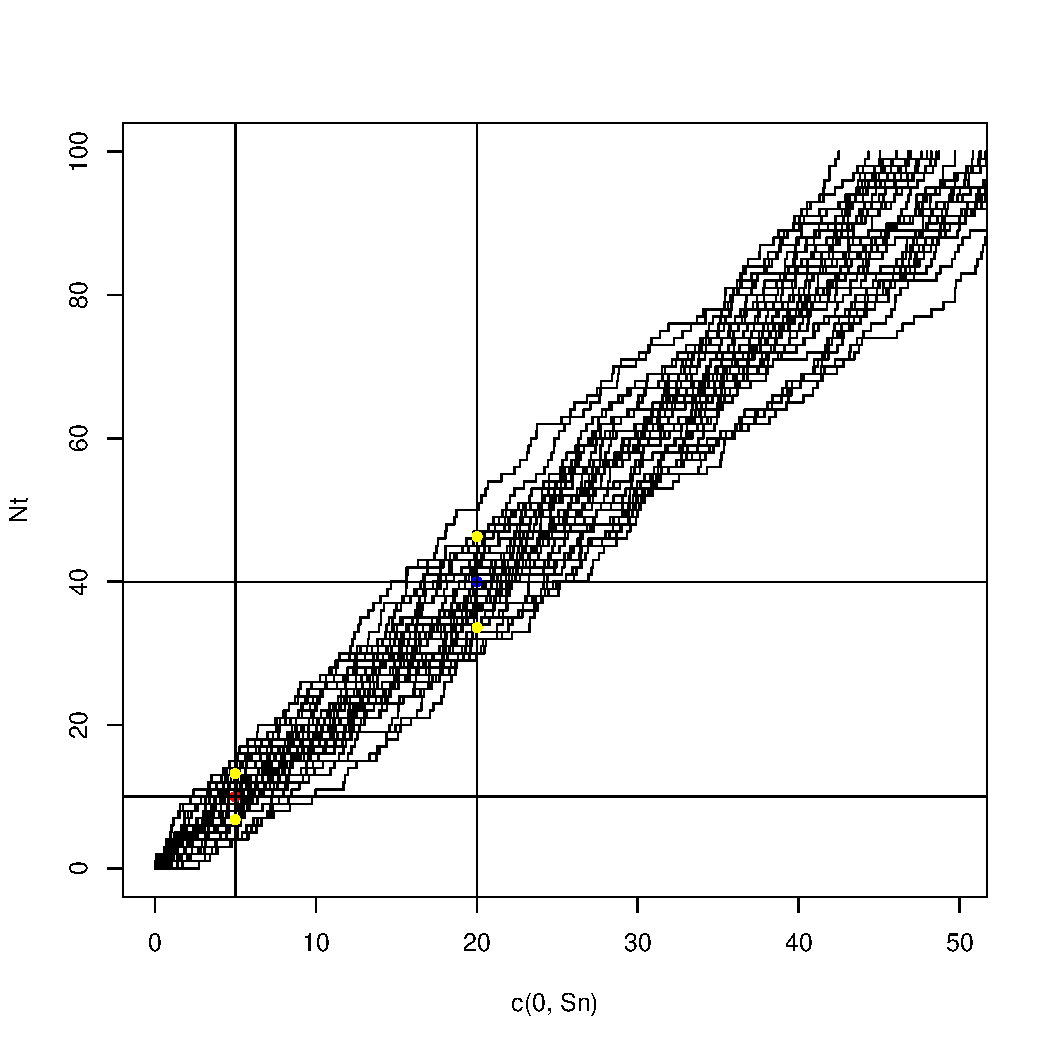
\includegraphics[scale=0.9,page=1]{Rplots3.pdf}
  \caption{30 indepentant realizations of poisson process with $\lambda = 2$}
  \label{poisproc}
\end{figure}

The red point shows the E(N(5)) and the blue point shows E(N(20)) which correspond nicely with the graph.

As for the standard deviation we can notice that it gets bigger when t0 gets bigger, and this is also visible on the graph with 30 instances, it gets spread out more as the number of observations increase.


\section*{Problem 4}

\subsection*{a)}
$T_1$  and $T_2$ are exponentially distributed with mean 1 becuse we are drawing from uniform distribution $U\sim U[0,1]$ and using inverse transform sampling.
ref \cite{referencja}
\subsection*{b)}

\begin{figure}[H]
  \centering
  \includegraphics[scale=0.5,page=2]{Rplots4.pdf}
  \caption{Scatter plot of $T_1$ vs $T_2$ with $\rho = -0.9$}
  \label{t1t2neg}
\end{figure}

\begin{figure}[H]
  \centering
  \includegraphics[scale=0.5,page=5]{Rplots4.pdf}
  \caption{Scatter plot of $T_1$ vs $T_2$ with $\rho = 0.9$}
  \label{t1t2pos}
\end{figure}

The corraletion estimate of $T_1$ and $T_2$ is

$cor(T_1,T_2) = -0.6$
when $\rho = -0.9$ and

$cor(T_1,T_2) = 0.88$
when $\rho = 0.9$

\begin{figure}[H]
  \centering
  \includegraphics[scale=0.5,page=3]{Rplots4.pdf}
  \caption{Scatter plot of $U_1 vs U_2$ with $\rho = -0.9$}
  \label{u1u2neg}
\end{figure}

\begin{figure}[H]
  \centering
  \includegraphics[scale=0.5,page=6]{Rplots4.pdf}
  \caption{Scatter plot of $U_1 vs U_2$ with $\rho = 0.9$}
  \label{u1u2pos}
\end{figure}


\begin{figure}[H]
  \centering
  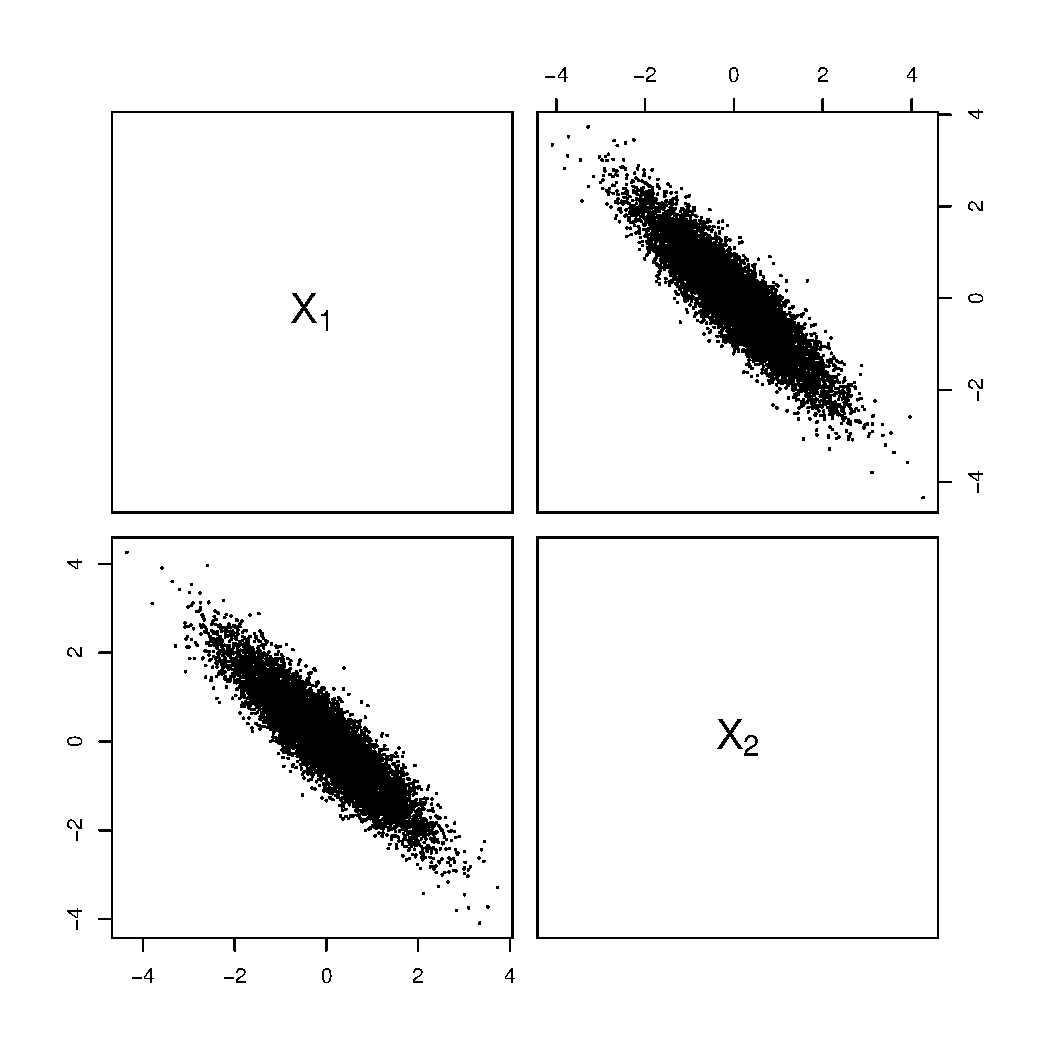
\includegraphics[scale=0.5,page=1]{Rplots4.pdf}
  \caption{Choleski faktorization gave strong negative visible corralation $\rho = -0.9$}
  \label{x1x2neg}
\end{figure}

\begin{figure}[H]
  \centering
  \includegraphics[scale=0.5,page=4]{Rplots4.pdf}
  \caption{Choleski faktorization gave strong positive visible corralation $\rho = 0.9$}
  \label{x1x2pos}
\end{figure}


\subsection*{c)}

\begin{figure}[H]
  \centering
  \includegraphics[scale=0.5,page=7]{Rplots4.pdf}
  \caption{Histogram of $Y=T_1 + T_2$ with $\rho = -0,9$, $P(Y\geq4) = 0.039$}
  \label{ygekroneg}
\end{figure}

\begin{figure}[H]
  \centering
  \includegraphics[scale=0.5,page=8]{Rplots4.pdf}
  \caption{Histogram of $Y=T_1 + T_2$ with $\rho = 0,9$, $P(Y\geq4) = 0.128$}
  \label{ygekropos}
\end{figure}

\subsection*{d)}
The estimate of $P(Y\geq4) = 0.04$ when $\rho = -0.9$

and $=0.131$ when $\rho = 0.9$ see Figure \ref{ygekroneg} and \ref{ygekropos}

\begin{lstlisting}
  mean(Y1>=4)/sqrt(n) #rho = -0.9
  mean(Y2>=4)/sqrt(n) #rho = 0.9
  >[1] 0.0019
  >[2] 0.0034
\end{lstlisting}

standard error is 0.0019 and 0.0034 for rho: -.9 and .9 respectively.\\

Corralation does not affect $E(Y) = E(T_1,T_2)$ ,

$cor(X,Y) = \frac{cov(X,Y)}{sd(X)sd(Y)}$ where $cov(X,Y) = E([X-E(X)][Y-E(Y)])$

ref \cite{referencja} corralation is dependent on E(Y)

\begin{thebibliography}{9}
  
\bibitem{referencja} 
  Lecture notes, and Rizzo material that relevant to the course.

\end{thebibliography}

\end{document}
